\documentclass[tikz]{standalone}
\usepackage{pgfplots}
\usepackage{amsmath}
\usepackage{xcolor}
\usetikzlibrary{calc}
\definecolor{blue}{HTML}{6d9eeb}
\definecolor{gray}{HTML}{888888}
\definecolor{gold}{HTML}{ffd966}
\definecolor{green}{HTML}{6aa84f}
\definecolor{purple}{HTML}{674ea7}
\pgfplotsset{compat=1.18}

\begin{document}
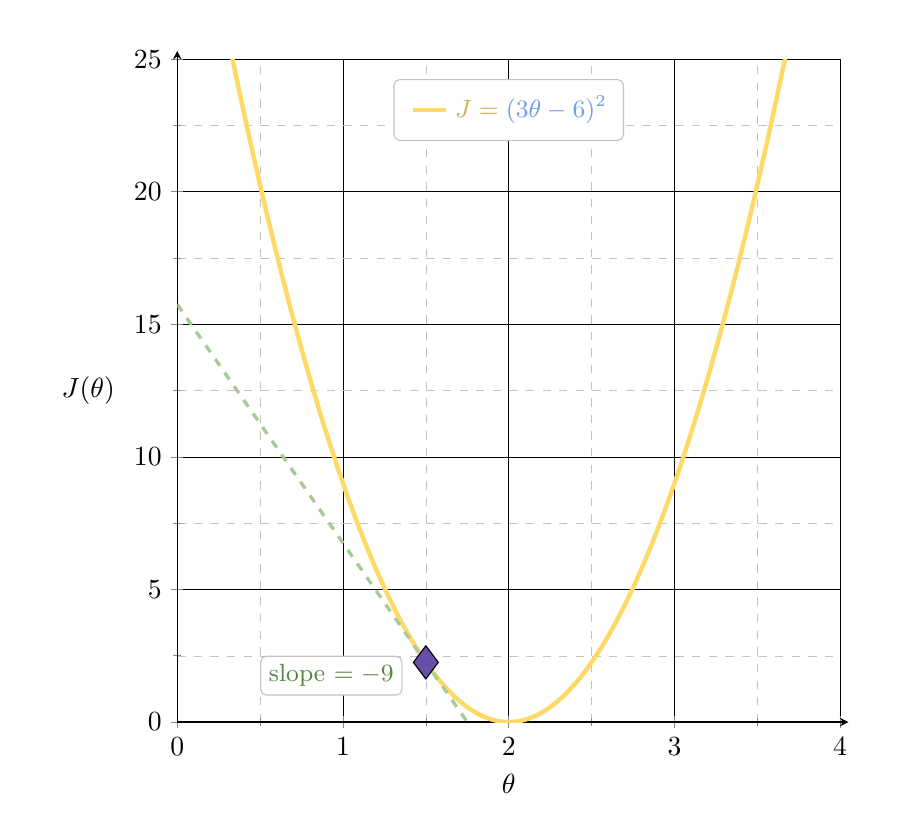
\begin{tikzpicture}
  \begin{axis}[
    set layers,
    axis lines=left,
    x axis line style={->,>=stealth, shorten >=-3pt},
    y axis line style={->,>=stealth, shorten >=-3pt},
    xlabel={\(\theta\)},
    ylabel={\(J(\theta)\)},
    ylabel style={rotate=-90},
    xmin=0, xmax=4,
    ymin=0, ymax=25,
    xtick={0,1,...,4},
    ytick={0,5,...,25},
    minor x tick num=1,
    minor y tick num=1,
    grid=both,
    major grid style={line width=0.2pt,draw=black},
    minor grid style={line width=0.1pt,draw=gray!50,dashed},
    width=10cm,
    height=10cm,
  ]
    % J(θ) = (3θ-6)^2
    \addplot[domain=0.33:3.67, samples=200, ultra thick, color=gold]
      {(3*x-6)^2};

    % Tangent line at θ=1.5: slope=-9, J(1.5)=2.25
    % y = 2.25 + (-9)(x - 1.5) = 15.75 - 9x
    \addplot[domain=0:4, samples=2, line width=1.2pt, color=green!60, dashed] {15.75 - 9*x};

    % Diamond marker at θ=1.5
    \addplot[only marks, mark=diamond*, mark options={scale=3, fill=purple}]
      coordinates {(1.5,2.25)};

    % Label with written-out expression
    \begin{pgfonlayer}{axis foreground}
    \node[gold!80!black, font=\small, anchor=north, fill=white, draw=gray!50, inner sep=6pt, rounded corners=2pt] at (axis cs:2,24.25)
      {\raisebox{0.5ex}{\tikz\draw[gold, ultra thick] (0,0) -- (0.2,0);}\;$J = \textcolor{blue}{(3\theta - 6)^2}$};
    % Slope annotation
    \node[green!80!black, font=\small, anchor=north west, fill=white, draw=gray!50, inner sep=3pt,
          rounded corners=2pt] at (axis cs:0.5,2.5) {slope $= -9$};
    \end{pgfonlayer}
  \end{axis}
  \pgfresetboundingbox
  \useasboundingbox ([xshift=-19mm, yshift=-11mm]current axis.south west)
    rectangle ([xshift=4mm, yshift=4mm]current axis.north east);
\end{tikzpicture}
\end{document}
